
% Provide some background on neural networks

\section{Neural networks}
\label{sec:networks}
\textit{
In this section, we first give an introduction to neural networks, especially convolutional neural networks, and then describe recent research in applying neural networks to tasks in computer vision.
For further reading about neural networks and applied deep learning, we recommend the detailed textbook by \textcite{GoodfellowBook}.
% For a more exhaustive reading of neural networks and deep learning we recommend the reader to search out a textbook in the field such as \cite{GoodfellowBook}.
}

\subsection{Introduction to neural networks}

Neural networks have recently gained popularity in various fields.
% They have been observed to be quite flexible in being able to classify data, find clusters and
% Neural networks can find meaningful information in a sea of data by clustering,
Applications include finding principal components, organizing meaningful clusters in a sea of data and generating new information, for example by translating natural languages \cite{machine_translation_attention}. Here, we will focus on the task of \textbf{classification}, which refers to choosing the correct class $y$ for some given input $\mathbf{x}$. For example to correctly recognize objects in an image or to select a strategic action to take in a game.

\subsubsection{Multilayer perceptron}

\begin{figure}
\centering
\begin{tikzpicture}

\tikzset{vertex/.style = {shape=circle,draw,minimum size=1.5em}}
\tikzset{edge/.style = {->,> = latex'}}

\node[vertex] (x1) at (0,0) {};
\node[vertex] (x2) at (0,1) {};
\node[vertex] (x3) at (0,2) {};
\node[vertex] (x4) at (0,3) {$x_k$};

\node[vertex] (v1) at (2,0.5) {};
\node[vertex] (v2) at (2,1.5) {};
\node[vertex] (v3) at (2,2.5) {$u_j$};

\node[vertex] (y1) at (4,0.5) {};
\node[vertex] (y2) at (4,1.5) {};
\node[vertex] (y3) at (4,2.5) {$v_i$};

\node[vertex] (o1) at (6,1) {};
\node[vertex] (o2) at (6,2) {$o_l$};

%edges
\draw[edge] (x1) to (v3);
\draw[edge] (x2) to (v3);
\draw[edge] (x3) to (v3);
\draw[edge] (x4) to (v3);

\draw[edge] (x1) to (v2);
\draw[edge] (x2) to (v2);
\draw[edge] (x3) to (v2);
\draw[edge] (x4) to (v2);

\draw[edge] (x1) to (v1);
\draw[edge] (x2) to (v1);
\draw[edge] (x3) to (v1);
\draw[edge] (x4) to (v1);

\draw[edge] (v1) to (y1);
\draw[edge] (v2) to (y1);
\draw[edge] (v3) to (y1);

\draw[edge] (v1) to (y2);
\draw[edge] (v2) to (y2);
\draw[edge] (v3) to (y2);

\draw[edge] (v1) to (y3);
\draw[edge] (v2) to (y3);
\draw[edge] (v3) to (y3);

\draw[edge] (y1) to (o1);
\draw[edge] (y2) to (o1);
\draw[edge] (y3) to (o1);

\draw[edge] (y1) to (o2);
\draw[edge] (y2) to (o2);
\draw[edge] (y3) to (o2);

\path[edge] (x4) -- node[above] {$w_{jk}$} (v3);
\path[edge] (v3) -- node[above] {$w_{ij}$} (y3);
\path[edge] (y3) -- node[above] {$w_{li}$} (o2);

\end{tikzpicture}

\caption{A multilayer perceptron with an input layer $x$, two hidden layers $u$ and $v$ as well as a readout layer $o$. Every connection uses a different weight $w$.}
\label{fig:mlp}
\end{figure}


A \textbf{multilayer perceptron} (MLP) is organized in several \textbf{layers}, see illustration in figure \ref{fig:mlp}. Each layer consists of a number of \textbf{neurons}.
%, the first layer has the same number as elements in the input vector $\mathbf{x}$.
Each element in the input vector $\mathbf{x}$ becomes a neuron in the \textbf{input layer}. Each neuron $v_i$ in the following layers gets its value by computing a weighted sum over the neurons $u_j$ in the previous layer using weights  $w_{ij}$, a bias term $b_i$ and an \textbf{activation function} $g$:

\[
v_i = g\left( b_i + \sum_j w_{ij} u_j \right)
\]

In order for the network to utilize the power of several layers, the activation function must be non-linear. If $g$ would be linear, then the entire network would be a series of linear transformations which could be rewritten as a single linear transformation. Traditional choices of $g$ include the hyperbolic tangent and the logistic function (which is sometimes referred to as the sigmoid function).

The final layer is called the \textbf{readout layer} and has as many neurons as there are classes. The input $\mathbf{x}$ is classified as the class $y$ which has the greatest value in the readout layer. In order to estimate the certainty, we can compute pseudo-probabilities $p_i$ of the classes by taking the \textbf{softmax} of the readout values $o_i$:

\[
p_i = \frac{ \exp(o_i) }{ \sum_k \exp(o_k) }
\]

The layers between the input layer and the readout layer are referred to as \textbf{hidden layers}.

\subsubsection{Backpropagation} \label{sssec:BackProp}

In order to correctly classify new input, we need to \textbf{train} the network on some existing data set $D$ which consists of pairs of correct classifications $(\mathbf{x}^{(\mu)}, y^{(\mu)}$).
We let $\mathbf{y}^{(\mu)}$ denote a \textbf{onehot} vector, that is all elements are zero except the indicated class whose associated element has the value one.
We then introduce a loss function $L$ to measure how different one network prediction $\mathbf{p}^{(\mu)}={\ldots, p_i^{(\mu)}, \ldots}$ is from its correct classification $\mathbf{y}^{(\mu)}$. Here we suggest the \textbf{squared error} loss function:

\[
L(\mu) = \frac{1}{2} \Vert
  \mathbf{y}^{(\mu)} - \mathbf{p}^{(\mu)}
\Vert ^2
\]

Given our loss function $L$, we can create a \textbf{cost} $H$ that represents the mean error over the data set $D$:

\[
H = \frac{1}{\vert D \vert} \sum_{\mu \in D} L(\mu)
\]

When $H$ is minimized, the network associates each input $\mathbf{x}^{(\mu)} \in D$ with the correct class. Since $H$ is differentiable, we can use standard \textbf{gradient descent} to optimize the network parameters, that is all weights $w_{ij}$ and biases $b_i$.
In iteration $k$ we use some \textbf{learning rate} $\eta$ and the gradient of the error $H$ to update the parameters $\mathbf{\theta}$:

\[
\mathbf{\theta}_{k+1} \leftarrow
\mathbf{\theta}_k - \eta \nabla_{\mathbf{\theta}} H
\]

\subsubsection{Stochastic gradient descent}

Since gradient descent is susceptible to local minima, it is common to use other optimization techniques such as \textbf{stochastic gradient descent} (SGD).
In gradient descent above, we let $H$ sum over all data points in $D$ in every iteration. In contrast, SGD draws a new random subset $B \subset D$ in each iteration. We refer to $B$ as a \textbf{mini-batch}. We then compute the cost $H$ as a sum over $B$ and use its gradient to update the network parameters:

\[
H = \frac{1}{\vert B \vert} \sum_{\mu \in B} L(\mu)
\]

\[
\mathbf{\theta}_{k+1} \leftarrow
\mathbf{\theta}_k - \eta \nabla_{\mathbf{\theta}} H(k)
\]

It is common to randomly partition $D$ into mini-batches so that all mini-batches are disjoint. Iterating over the entire dataset is then referred to as an \textbf{epoch}.
The random partition of $D$ should be different for each new epoch.
To achieve the wanted accuracy, it is often necessary to train over many epochs.


\subsubsection{Testing and evaluating}

Because neural networks have many parameters, they risk memorizing the training data and hence fail to learn the general patterns that we actually want them to recognize.
% \cite{AlexNet, FornesCnnCategorization}.
This phenomenon is knows as \textbf{overfitting} and can constitute a large problem for small datasets. In order to estimate overfitting, we divide the original dataset into one part for training and one for testing. The training data is used for backpropagation while the test data is exclusively used for testing. If the network begins to overfit on the training data, the accuracy on the test data decreases and the training should be aborted.

It is also common to have a third data set for evaluation which is disjoint with both the training data and the test data.


\subsection{Deep neural networks}
% Very powerful, see for example AlphaGo
% Many parameters, needs lot of data

One of the reasons why neural networks have recently achieved state-of-the-art in so many tasks is the use of very deep networks, that is networks with many layers.
% TODO add citation
The more layers, the more complex tasks can be learned. To the surprise of many, computers recently even outperformed humans in the complex game of Go \cite{AlphaGo, AlphaGoTuringTest}.

The large number of parameters in deep networks is both a strength and a weakness since it requires a large amount of training data as well as considerable computation power. More parameters can also memorize more and thus make the network more prone to overfitting \cite{AlexNet}.

\subsubsection{Dropout}

One way to reduce the risk of overfitting is by applying \textbf{dropout}  \cite{AlexNet, FornesCnnCategorization}.
%Another problem with large networks is overfitting which means that the network learns the training set by heart instead of learning to recognize the general patterns \cite{AlexNet, FornesCnnCategorization}.
The dropout method introduces a probability of setting each neuron's activation to $0$ during training, often with $50\%$ probability. This forces the network to learn multiple paths for recognizing different features and hence creating a more robust representation. Dropout also reduces the computational cost because fewer neurons participate in each training step.
Note that dropout is not necessarily done for every layer in the network.


\subsubsection{Weight decay}

Another common technique to avoid overfitting is \textbf{weight decay} \cite[Chapter~3]{NielsenBook} \cite[Chapter~7]{GoodfellowBook}. We add a new penalty term for weight regularization to our previous cost $H$, where $\mathbf{w}$ denotes all weight parameters $w_{ij}$ but not the bias parameters $b_i$:

\[
\tilde{H} = H + \alpha \Omega(\mathbf{w})
\]

The amount of regularization is determined by the hyper-parameter $\alpha \in [0,\infty)$.
A common version of weight decay is \textbf{L2 regularization}:

\[
\Omega(\mathbf{w}) = \frac{1}{2} \mathbf{w}^T \mathbf{w}
\]

By computing the gradient for the new cost metric $\tilde{H}$, we get the new update rule for the weights:

\[
\mathbf{w}_{k+1} \leftarrow
(1 - \eta \alpha) \mathbf{w}_k - \eta \nabla_{\mathbf{\theta}} H(k)
\]

We see that $\mathbf{w}$ decays with a factor $(1 - \eta \alpha)$ in each iteration, so the weights decay exponentially over time. Thus the weight decay makes sure that the weights are kept small no matter for how long the network is trained, that is no weight parameter can grow indefinitely. Empirically, it has been observed that networks can be trained longer without overfitting when the weights are bounded \cite[Chapter~3]{NielsenBook}.

Since the penalty term does not include the bias terms, the update rule for the bias parameters is unchanged.


\subsubsection{Cross-entropy loss} \label{sssec:CrossEntropy}

Above in section \ref{sssec:BackProp}, we used squared error as the loss function $L$. One of the problems with squared error is that a large error does not always result in a large gradient \cite[Chapter~3]{NielsenBook}.
A more commonly used loss function is \textbf{cross-entropy}, which has the property that its gradient depends directly on the distance between the network output and the correct value.
Thus in most cases, cross-entropy is a better choice as loss function than squared error.

For training example $\mu \in D$, we denote the network output in neuron $i$ as $p_i^(\mu)$, while $y_i^(\mu)$ takes the value one if $i$ is the correct class and the value zero otherwise. Then we can define the cross-entropy loss $L$ as:

\[
L(\mu) = - \sum_i \left(
  y_i^(\mu) \log p_i^(\mu) + (1 - y_i(^\mu)) \log (1 - p_i^(\mu))
\right)
\]

This expression may not intuitively make sense as a loss function but we can make the following observations:

\begin{itemize}
    \item Because $p_i \in (0, 1)$, both $\log p_i$ and $\log (1 - p_i)$ must be negative and thus each term in the sum is negative. We have a minus sign before the sum, so $L(\mu)$ must be positive.
    \item The correct label $y_i$ can only take the value $0$ or $1$. If $y_i=1$, then the expression can be simplified as $\log p_i$ which is greater the farther $p_i$ is from the desired value $1$. By symmetry, the same holds for when $y_i = 0$.
\end{itemize}

In conclusion we can observe that $L(\mu) \geq 0$ and is minimized when the $y_i$ predict the correct label. Furthermore, the amplitude of the loss depends directly on how far away the actual output $p_i$ is from the expected output $y_i$. Therefore, cross-entropy has the properties of a good loss function.

\subsubsection{Momentum}

One problem with stochastic gradient descent (SGD) is that the learning can zig-zag across valleys in the optimization plane, especially for noisy gradients \cite[Chapter~8]{GoodfellowBook}. Another problem is that the learning becomes very slow for stable but small gradients. A suggested solutions to both problems is the use of \textbf{momentum}. When training with momentum, instead of directly updating the parameters $\mathbf{\theta}$, we apply the gradients to a decaying momentum $\mathbf{v}$:

\[
\mathbf{v} \leftarrow \alpha \mathbf{v} - \eta \nabla_{\mathbf{\theta}} H
\]

The accumulated momentum is then applied to update the parameters:

\[
\mathbf{\theta} \leftarrow \mathbf{\theta} + \mathbf{v}
\]

With momentum, the learning no longer zig-zags across valleys because the accumulated momentum would point directly in the direction of the valley. For stable but small gradients, the learning would accelerate because the accumulated momentum grows in the same direction. Thus both problems presented above are mitigated by momentum.

\subsubsection{Alternative learning algorithms}

Although SGD is a very common technique to minimize the cost $H$, there are several popular alternatives. In stochastic gradient descent, the learning rate is a fixed hyper-parameter $\eta$ that is set manually by the programmer and is often adjusted after considerable empirical experimentation. A too high learning rate may overshoot the optimal values and hinder convergence while a too small learning rate may unnecessarily cause a long training time.

For many tasks it is desirable that the learning rate is high in the beginning when the network is very wrong while the learning rate should be small at the end when the distance to the optimal solution is small. There are several popular methods that use an adaptive learning rate: \textbf{AdaGrad}, \textbf{RMSProp} and \textbf{Adam} \cite[Chapter~8]{GoodfellowBook}. However, there is no clear consensus about which method is the best. People seem to prefer the method they are used to since their personal experience helps with setting the hyper-parameters.

Although gradient-based methods dominate the field, it is not the only possible approach. \textbf{Particle swarm optimization} has also been suggested for training neural networks in cases when it may be difficult to compute the gradient \cite[Chapter~5]{StochasticOpt}.

\subsubsection{Rectified linear activation}

Very deep networks suffer from the \textbf{vanishing gradient} problem.
Backpropagation updates each parameter according to its gradient but if the gradient is very small, it will take a long time before the network converges.
Such small gradients can occur when using the traditional activation functions, hyperbolic tangent and the logistic function, because they have very small gradients for large activations \cite{AlexNet}.
This can largely be solved by using the \textbf{rectified linear} (ReLU) function for activation: $g(x) = \max \{0, x\}$.


\subsubsection{Pre-training and transfer learning}

When the intended task has limited training data or takes a long time to train, it can be useful to start with a network that has already been trained on a different task or data set.
For example, \cite{SpatialTransformerNetworks} use the Inception network pre-trained on ImageNet.
The idea is that the parameters in a network trained on a related task is probably closer to their optimal value than randomly initialized parameters. For example, recognizing edges and corners are central to many visual recognition tasks.

% TODO: is this accurate? Book also mentions greedy pre-training such as training some layers at a time?

\subsection{Deep learning in computer vision}

Both machine translation and image captioning used to be solved by solving each subproblem separately but this kind of approach has been outperformed by end-to-end systems using deep learning \cite{ShowAndTell}. One neural network \textbf{encoded} the input to a fixed-length vector representation which was \textbf{decoded} by another network. In the case of machine translation both the encoder and decoder was implemented by an RNN which are highly suitable for processing sequences like sentences. The image captioning system was implemented in a similar manner but using a \textbf{convolutional neural network} (CNN) as encoder.


\subsection{Convolutional neural networks}

Since the publication of the AlexNet in 2012 \cite{AlexNet}, CNNs have gained large attention in computer vision for achieving state-of-the-art in various tasks such as object-detection, segmentation, video classification and object tracking \cite{InceptionV3}.

\begin{figure}
\centering

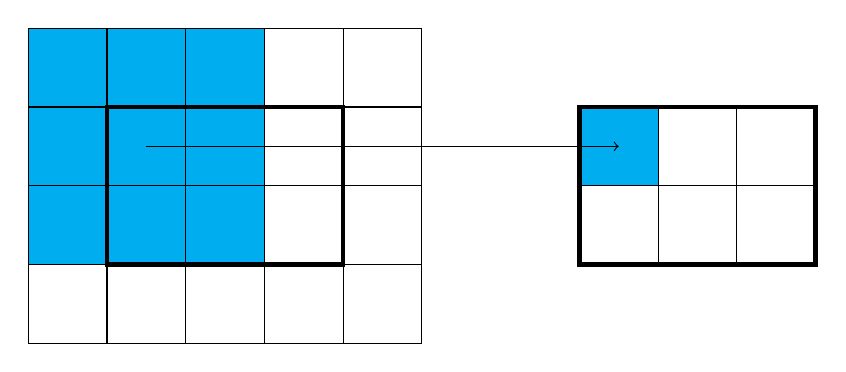
\begin{tikzpicture}
%  , fill=black!20!white
\draw [draw=black, fill=cyan] (0,1) rectangle (3,4);
\draw [draw=black, ultra thick] (1,1) rectangle (4,3);
\draw [draw=black] (0,0) grid  (5,4);

\draw [draw=black, fill=cyan] (7,2) rectangle (8,3);
\draw [draw=black, ultra thick] (7,1) rectangle (10,3);
\draw [draw=black] (7,1) grid  (10,3);

% ,very thick
\draw [->] (1.5, 2.5) -- (7.5, 2.5) ;

\end{tikzpicture}

\caption{Applying a $3 \times 3$ filter to a layer of size $4 \times 5 \times 1$. Note how the $3 \times 3$ region is reduced to a single unit and how the size of the activation map is decreased after the operation.}
\label{fig:filter}
\end{figure}


% TODO add citations

In CNNs, each layer has a width, height and depth. Like in MLPs, the input layer has the width and height of the input image while the depth correspond to the number of color channels (one for gray scale, three for RGB and four for RGBA). We now refer to each number in the network as a \textbf{unit} instead of a neuron.

As indicated by the name, CNNs mainly consist of \textbf{convolutional layers}. The depth of a convolutional layer is determined by how many filters it has. Each filter produces a two-dimensional \textbf{activation map}, see figure \ref{fig:filter}. Each unit in the activation map comes from a weighted sum over a three-dimensional region in the previous layer over its full depth. For example a $3 \times 3$ filter applied to a 32 depth layer has $3 \cdot 3 \cdot 32=288$ weights and one bias term.
Like with MLP, the sum is passed to to a non-linear activation function such as $\tanh$. The $3 \times 3$ regions for each unit are overlapping.
The activation maps for all filters are stacked together to form a three-dimensional output, which is passed to the next layer.

Because a filter uses the same weights for all sub-regions in the previous layer, the total number of parameters are dramatically reduced compared with a fully connected layer as in an MLP. Moreover, because the same filter is applied to each sub-region, it does not matter where in the input image the object is located.

Units in higher layers in the CNN receive information from a larger \textbf{receptive field} in the input image.
% Each $2 \times 2$ pooling layer doubles the receptive field in each dimension, while every $3 \times 3$ convolutional layer increases the receptive field with 2.
Therefore, the filters in lower layers typically learn to detect low-level features like edges and curves while filters in higher layers can detect more complex objects like cats or faces.
By synthesizing the input image to maximize a specific filter's activation, it is possible to get an idea of what the filter has learned to recognize \cite{VisualizeCnn}.

\begin{figure}
\centering
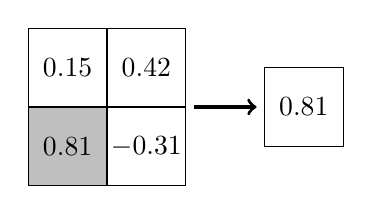
\begin{tikzpicture}

\fill[draw=black,color=lightgray] (0,0) rectangle (1,1);
\draw (0,0) rectangle (1,1) node[pos=0.5] {$0.81$};
\draw (0,1) rectangle (1,2) node[pos=0.5] {$0.15$};
\draw (1,0) rectangle (2,1) node[pos=0.5] {$-0.31$};
\draw (1,1) rectangle (2,2) node[pos=0.5] {$0.42$};

\draw (3,0.5) rectangle (4,1.5) node[pos=0.5] {$0.81$};
\draw [->,very thick] (2.1,1) -- (2.9,1) ;

\end{tikzpicture}

\caption{Example of a $2 \times 2$ max pool operation. In a $2 \times 2$ region, the largest value is chosen while the other values are ignored.}
\label{fig:maxpool}
\end{figure}


Besides filters, CNNs also use \textbf{pooling layers} in order to increase the receptive field without increasing the number of parameters in the model.
Separately for each activation map, pooling aggregates a two-dimensional region of units (e.g. $2 \times 2$) into a single unit, typically by taking the maximum value; see figure \ref{fig:maxpool}. These regions are non-overlapping so a $2 \times 2$ pooling layer decreases the representational size by 4. Thus another benefit of pooling layers is reduced computation time.

We can calculate the size of the receptive field for each output unit by doubling the field for each $2 \times 2$ pooling layer and adding $n-1$ for each $n \times n$ convolutional layer.
If we have a network that consists of two $5 \times 5$ convolutional layers with a single $2 \times 2$ maxpool layer in between, then we can compute the pixel size $r \times r$ of the receptive field as follows:

\[
r = 4 + 2(4 + 1) = 14
\]

At the end of the network, there are often a few fully connected layers (MLP) where the last layer represent the output of the network, for example pseudo-probabilities for different categories using softmax like discussed previously.

\subsubsection{Network architecture for faster computation}

The performance of CNNs typically increases with greater width and depth but it comes at a higher computational cost \cite{InceptionV3}. However, by choosing a good network architecture the same performance can be achieved but at a substantially lower computational cost, for example by refactoring large filters ($5 \times 5$, 7x7) into consecutive small filters ($3 \times 3$) and extensive use of pooling layers to reduce dimensionality. The authors also suggest a balance between depth and width of the network.

\subsubsection{Zero padding}

Applying a $3 \times 3$ filter to an input image of size 10x10 will output an image of size 8x8 since there are only 8 positions in a single row where the filter can fit. For deep networks, this shrinking might cause the final representation to become too narrow.
One can pad each activation map with zeroes to instead maintain the same size.

\subsection{Attention models}
\label{ssec:attention}
% Since waypointing only needs high-level information in a limited domain, complete transcription is unnecessary. Instead we can use recent advances in image classification.

% TODO write this part again in more detail, especially after spending more time with the literature here.

In contrast to CNNs, the human eye doesn't process the entire scene with equal precision but focuses on the most relevant parts \cite{DeepMindAttention}.
Similarly, we can let the system pay \textbf{attention} to a small part of the image at a time and successively increase the system's understanding of the image.
By choosing good locations for our attention, the important parts of the image are captured while ignoring irrelevant parts.
This reduces the computation time for training and also increases the precision of the network.
% The process of how to select a location to focus on is called an \textbf{attention model} and is often implemented using a \textbf{recurrent neural network} (RNN).
Besides image classification, attention models have also been highly successful for image captioning \cite{AttendAndTell} and machine translation \cite{machine_translation_attention}.

\subsubsection{Details}
We now describe how the attention model in \cite{AttendAndTell} works in more detail.
The goal of the attention model is to produce a vector $\mathbf{z} \in \mathbb{R}^D$ that represents the entire input image by weighing different parts of the output from the encoder CNN.

The encoder output is three-dimensional but can be seen as a grid of $L$ feature vectors. Each feature vector $\mathbf{a_i} \in \mathbb{R}^D$ corresponds to a specific location in the input image. We feed each $\mathbf{a_i}$ to an MLP which produces a scalar $e_i \in \mathbb{R}$. In the paper, the decoder uses an RNN whose hidden state is also used as input to the MLP besides the feature vector $\mathbf{a_i}$.
The scalar attention weight $\alpha_i$ for each location can then be computed by taking the softmax of $e_i$ over all units:

\[
\alpha_i = \frac{ \exp(e_i) }{ \sum_{k=1}^L \exp(e_i) }
\]

\paragraph{Soft attention}
By definition, the attention weights sum to one. A \textbf{soft attention} model computes the representative vector $\mathbf{z}$ by summing over the feature vectors $\mathbf{a_i}$, using attention as weights:

\[
\mathbf{z} = \sum_{k=1}^L \alpha_i \mathbf{a_i}
\]

\paragraph{Hard attention}
In contrast, a \textbf{hard attention} model interprets the ${\alpha_i}$ as a probability distribution over locations $i$. By sampling this distribution, $\mathbf{z}$ is chosen to be the sampled unit $\mathbf{a_i}$, ignoring the rest of the image.


\subsection{CNNs in multi-digit recognition}

Digit recognition has been studied extensively, especially for recognition of zip-codes in the US postal service \cite{lecun_1989, lecun_1990}. Originally, the digits were segmented manually and linearly transformed to a fix input size of 16x16 pixels.
Each digit image was then classified using a CNN with 3 or 4 hidden layers, with $2 \times 2$ pooling between each convolutional layer.

A complete zip-code recognition system locates the place of the zip-code and segments the zip-code into digit images \cite{zipcode_system}. The segmentation is performed by finding \textbf{connected components} (CC) in the image. If the CC has a high confidence in classification it is removed, otherwise it is either split or combined with adjacent CCs until a segmentation has been found where each classification has a high enough confidence. This is done by building a directed acyclic graph where each proposed segment is a node. The length of a path is defined as the product of the classification confidence for each node in the path. The best segmentation is then the path of greatest length in the graph. In order to avoid redundant computations, the segmentation can be done indirectly after the convolutional layers instead of on the input image \cite{lecun_multidigit}.

More recently, deep neural networks have achieved state-of-the-art in multi-digit recognition in street view images \cite{multidigit_streetview}. Instead of handling localization, segmentation and classification as separate tasks, they solve all of them using a single CNN with 11 layers. The output is modeled as a sequence $S$ of digits with a maximum length $N$. The sequence $S$ consists of a random variable $L=n$ for the length of the sequence and $n$ variables $S_i$, one for each digit. In order to handle images without numbers $L$ is allowed to have the value zero and in order to handle longer sequences than $N$, $L$ has a special value "greater than $N$". For an input image $X$, the system can be trained by maximizing $\log P(S \vert X)$. Classification is similarly done by $\text{argmax}_S P(S \vert X)$.
Because each variable has a very small domain, they can be implemented with independent softmax outputs.
Although this model works well for digit recognition of short sequences $N \leq 5$ as well as OCR in CAPTCHAs, the authors speculate that the method is not suitable for long or unbounded sequences.

Another suggested approach to digit recognition in street view is to combine CNNs with HMMs \cite{multidigit_streetview_CNN_HMM}. They use a sliding window to extract multiple overlapping frames on the input image, classify each frame using a CNN to either a digit or null and then feed the sequence of frame labels to an HMM.



\subsection{Additional topics}

Here we list some additional recent progress in the field of neural networks in computer vision which is not used in the thesis.

\subsubsection{Confidence thresholding}

Certain tasks, like automatic house number transcriptions in Google Street View, require the model to have a very high accuracy to be useful \cite{multidigit_streetview}.
For these instances, the model should output a \textbf{confidence} for its classification. If the confidence is higher than some pre-determined threshold $\tau$, we keep the prediction; otherwise we ignore the prediction and conclude that the model is not sure about that example.
% In order to increase the accuracy, the predictions that have a confidence lower than some threshold $\tau$ may be discarded.
We then need to use two metrics for evaluating the model's performance: \textbf{precision} and \textbf{recall}.

The precision measures the quality of the predictions that were higher than the threshold. It is the accuracy, or percentage of correct predictions, among the predictions that were not discarded.
% Out of the non-discarded predictions, the precision is the percentage of correct predictions.

Recall on the other hand measures how many correct predictions were discarded due to low confidence. Instead of measuring recall, we can use \textbf{coverage}, which is simply the percentage of predictions whose confidence was above the threshold $\tau$.
% TODO: is it really?
% More precisely, recall is the number of correct predictions that were not discarded divided by the total number of correct predictions.

In order to compare models, we can then plot precision vs recall or coverage for different values of $\tau$. For $\tau=0$, the precision is the same as accuracy and the coverage is $100\%$. For $\tau=1.0$, everything is discarded so the precision is $100\%$ but the coverage is $0\%$.

\subsubsection{Batch normalization}

An alternative to Dropout was suggested by \cite{BatchNormalization}. Besides reducing the risk for overfitting, the authors also suggest that it allows for a higher learning rate in deep networks and thus faster convergence.

For some network layer $\mathbf{x} = {x_1, \ldots, x_d}$, we normalize each $x_i$ to zero mean and unit variance over the current mini-batch:

\[
\hat{x_i} = \frac{x_i - E[x_i]}{ \sqrt{\text{Var} [x_i]} }
\]

We then use two learned parameters $\gamma$ and $\beta$ to instead output $z_i$:

\[
z_i = \gamma \hat{x_i} + \beta
\]

The batch normalization can thus be summarized as $\mathbf{z} = f_{BN}(\mathbf{x}; \gamma, \beta)$.

The batch normalization can either be applied before or after the activation function. The authors suggest that the best result is achieved by applying the batch normalization before the non-liner activation $g$ but after the weights $w_{ij}$ and bias $b_i$:

\[
v_i = g\left( f_{BN}\left( b_i + \sum_j w_{ij} u_j; \gamma, \beta \right) \right)
\]

\subsubsection{Visual-semantic alignment}

% Another way to model regions in the input is by using a R-CNN which have also been very successful at image captioning

Another successful approach to image captioning uses a \textbf{region convolutional neural network} (R-CNN) as encoder \cite{VisualSemanticAlignment}.
The original R-CNN method works by proposing 2000 regions in the image that are the most likely to contain an object \cite{RCNN}. Each region is then fed to a regular CNN for encoding before classification.

Since many regions overlap, it is unnecessary to compute the convolutions for them independently \cite{FastRCNN}. Instead the entire input image is processed through the CNN once and the feature vector of each region is extracted from the resulting activation map. After this improvement, the bottleneck is selecting the regions \cite{FasterRCNN}. By making a neural network to select regions from the activation map instead of from the image, the computation speed can be significantly reduced. However, this requires the training data to contain bounding boxes for the objects to detect.

In the case of image captioning, the correspondences between words and regions in the image is unknown so this relationship is modeled by latent variables \cite{VisualSemanticAlignment}.

\subsubsection{Spatial pyramid pooling}

Convolutional layers and pooling layers can handle input images of changing sizes since the filters just slide over the entire image, so the size of the output matches the input.
However, because the last layers are fully connected, they can only handle input of a fixed size. A common solution to this is to rescale or crop the input \cite{FornesCnnCategorization}. If the input consists of segmented images of handwritten words then cropping will cut away critical information while rescaling risk distorting the handwriting beyond recognition. A proposed solution to this is using a layer of \textbf{spatial pyramid pooling} (SPP).
% TODO describe SPP in more detail if relevant

\subsubsection{Spatial transformer networks}

% TODO describe Spatial transformer networks and what they are good for.
% \cite{SpatialTransformerNetworks}

\subsubsection{Residual networks}

% TODO cite Microsoft ResNet for architecture of Residual modules. There are also residual networks of residual networks.
